\subsection{MSVC + \olly}
\index{\olly}
\RU{Проиллюстрируем всё это в}\EN{Let's illustrate this in} \olly.
\RU{Когда мы протрассируем до первой инструкции в \ttf, которая использует какой-то из аргументов
(первый), мы увидим, что \EBP указывает на \glslink{stack frame}{фрейм стека}, 
я выделил его красным прямоугольником.}
\EN{When we trace until the very first instruction in \ttf that uses one of the arguments 
(first one), we see that \EBP is pointing to the \gls{stack frame}, 
I marked it with red rectangle.}
\RU{Самый первый элемент \glslink{stack frame}{фрейма стека} --- это сохраненное значение \EBP, 
затем \ac{RA}, третий элемент это
первый аргумент ф-ции, затем второй аргумент и третий}\EN{The first element of \gls{stack frame} is saved \EBP value, 
second is \ac{RA}, third is first function argument, then second argument and third one}.
\RU{Для доступа к первому аргументу ф-ции, нужно прибавить к \EBP аккурат 8 (2 32-битных слова)}
\EN{To access the first function argument, one need to add exactly 8 (2 32-bit words) to \EBP}.

\olly \EN{is aware about this, so it added comments to stack elements like}
\RU{в курсе этого, так что он добавил комментарии к элементам стека вроде}
``RETURN from'' \AndENRU ``Arg1 = \dots'', \EN{etc.}\RU{и т.д.}

N.B.: \EN{function arguments are not members of function's stack frame, they are rather
members of stack frame of \gls{caller} function.}
\RU{аргументы функции являются членами фрейма стека вызывающей ф-ции а не текущей.}
\EN{Hence, \olly marked ``Arg'' elements as members of another stack frame.}
\RU{Поэтому \olly отметила элементы ``Arg'' как члены другого фрейма стека.}

\begin{figure}[H]
\centering
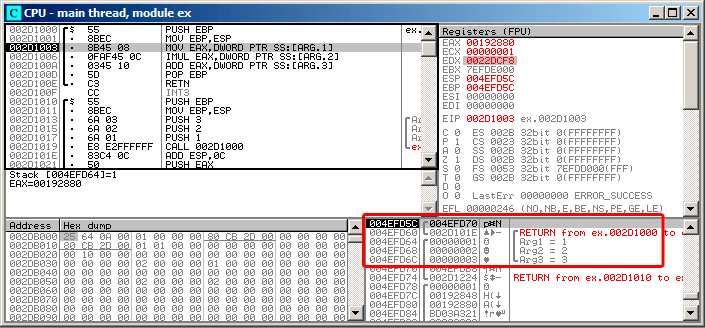
\includegraphics[scale=\FigScale]{patterns/05_passing_arguments/olly.png}
\caption{\olly: \RU{внутри ф-ции}\EN{inside of} \ttf{}\EN{ function}}
\label{fig:passing_arguments_olly}
\end{figure}
